
\chapter{Fixed-wing Unmanned Aerial Vehicles}\label{cha:fixed_wing_uav}
\section{General definitions and terminology}
Fixed-wind UAVs are receiving increasing commercial and research interest, and offer a number of advantages in many use-cases. In the following sections a thorough description of
general fixed-wing kinematics and control as well as a description of the specific platform used in this work will be presented. 
We begin with establishing some common definitions and terminology which will be used throughout this thesis. These definitions are 
 used in many other works related to fixed-wing aircraft, such as \cite{uav_dynamics_wind}. 

\subsection{Coordinate reference frames}
Four different coordinate frames are relevant to consider for UAV applications in wind: the inertial frame which is 
fixed in the earth, the air-relative frame, the body frame and the wind reference frame. The body frame and wind reference frames are related through the \textit{angle of attack} $\alpha$ and \textit{sideslip} $\beta$
 as shown in Figure \ref{fig:body_wind_frame}.
\begin{figure}
    \begin{center}
        \begin{tikzpicture}
            \coordinate (body) at ($(0,0)+(45:-.25)$);
            

            \draw[my_v] (body) -- node[at end, left]{$x$} (45:1.5);
            \draw[my_v] (body) -- node[at end, below]{$y$} (-45:1.5);

            \draw[my_v] (body) -- node[at end, left]{$x_{w}$} ++ (80:1.5);
            \draw[my_v] (body) -- node[at end, below]{$y_{w}$} ++ (-10:1.5);
            \draw[my_v] (body) -- node[at end, left]{$\vec{v}_I$} ++ (80:3);

            \draw[my_v] (.5,.5) arc(45:80:1) node[midway, anchor=225]{$\beta$};

            \Drone{0}{0}{50};
        \end{tikzpicture}
        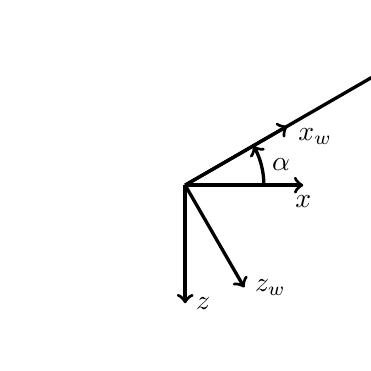
\begin{tikzpicture}
            \useasboundingbox (-2, -2) rectangle (2, 2);
            \coordinate (origin) at (0,0);

            \draw[my_v] (origin) -- node[at end, below]{$x$} ++ (1.5,0);
            \draw[my_v] (origin) -- node[at end, right]{$z$} ++ (0,-1.5);

            \draw[my_v] (origin) --node[at end, anchor=160]{$x_w$} ++ (30:1.5);
            \draw[my_v] (origin) --node[at end, right]{$z_w$} ++ (-60:1.5);
            \draw[my_v] (origin) --node[at end, anchor=160]{$\vec{v}_I$} ++ (30:3);

            \draw[my_v] (1,0) arc(0:30:1) node[midway, anchor=180]{$\alpha$};
        \end{tikzpicture}
    \end{center}
    \caption{Relation between body and wind frames}
    \label{fig:body_wind_frame}
\end{figure}

\begin{definition}[Inertial frame]
    The inertial frame, denoted with subscript $I$ is fixed relative to the earth.
    A position vector in the inertial frame is defined in the NED order as
    \begin{equation}
        \vec{p}_I = (x_N, y_E, -z_H)
    \end{equation}
    where $x_N$ points in the north direction, $y_E$ points east and $z_H$ points down towards the earth,
    in order to form a right hand positive coordinate system.
\end{definition}

\begin{definition}[Air frame]
    The air frame, denoted with subscript $A$ is fixed in the air and aligned with the current direction of wind. In the case of non-zero wind,
    this coordinate frame moves with the same speed.
    This means that inertial frame coordinates become time-dependent in the air frame, and are given by
    \begin{align}
        p_{N,A}(t) &= \cos\psi_w p_{N,I} + \sin\psi_w p_{E,I} - Wt\\
        p_{E,A}(t) &= -\sin\psi_w p_{N,I} + \cos\psi_w p_{E,I}
    \end{align}
    where $W$ is the wind speed and $\psi_w$ the wind direction.
\end{definition}

\begin{definition}[Body frame]
    The body frame, denoted with subscript $B$ is fixed in the UAV center of gravity.
    A position vector in the body frame is defined as
    \begin{equation}
        \vec{p}_B = (x, y, z)
    \end{equation}
    where $x$ points forward through the UAV, $y$ points to the right and $z$ points down.
\end{definition}

\begin{definition}[Wind reference frame]
    The wind reference frame, denoted with subscript $W$ is related to the current direction of motion
    through the air.
    A position vector in the wind reference frame is defined as
    \begin{equation}
        \vec{p}_W = (x_w, y_w, z_w)
    \end{equation}
    where $x_w$ points in the same direction as the current velocity vector $\vec{v}_I$, 
    $y_w$ points to the right of $x_w$ and $z$ points down relative $x_w$ and $y_w$.
\end{definition}

\subsection{Attitude representation}
The attitude of the UAV is represented by the \textit{Euler angles}. 

\begin{definition}[Euler angles]
The Euler angle vector is defined as
\begin{equation}
    \vec{\Phi}=(\phi, \theta, \psi)
\end{equation}
where the \textit{roll angle} $\phi$ is rotation around the north inertial axis, 
the \textit{pitch angle} $\theta$ is rotation around the east inertial axis and
the \textit{yaw angle} $\psi$ is rotation around the downwards inertial axis.

The relationship between coordinates in the body frame and inertial frame is given
in \cite{sensor_fusion} as the rotation matrix 

\begin{equation}\label{eq:r_i_b}
\mathcal{R}^I_B = \mathcal{R}^x_\phi\mathcal{R}^y_\theta\mathcal{R}^z_\psi\\
=
\begin{bmatrix}
    1 & 0 & 0 \\
    0 & \cos\phi & \sin\phi \\
    0 & -\sin\phi & \cos\phi
\end{bmatrix}
\begin{bmatrix}
    \cos\theta & 0 & -\sin\theta \\
    0 & 1 & 0 \\
    \sin\theta & 0 & \cos\theta
\end{bmatrix}      
\begin{bmatrix}
    \cos\psi & \sin\psi & 0 \\
    -\sin\psi & \cos\psi & 0 \\
    0 & 0 & 1
\end{bmatrix}
\end{equation}  
\end{definition}

This attitude representation is not defined for $\theta=\pm\pi/2$.

\subsection{Fixed-wing UAV}
A fixed-wing UAV is equipped with two horizontal wings that are fixed in the body frame.
In order to stay in the air, it needs to keep a minimum forward velocity
\begin{equation}
    V > V_{s}
\end{equation}
where $V_s$ is the airframe-dependent \textit{stall speed}. In order to navigate through the
air, it is equipped with some or all of the following control surfaces:
\begin{itemize}
    \item \textit{Ailerons} to control $\phi$
    \item \textit{Elevators} to control $\theta$
    \item \textit{Rudders} to control $\psi$
\end{itemize}
The UAV is also equipped with one or several propellers that are used to create the thrust which
increases the total energy of the system. These might be facing towards or against the direction of motion.


\section{Trajectory following}
In trajectory following, the goal is for the UAV to follow some pre-defined trajectory, which is a set of 
linear or curved segments in the inertial frame. This can be formulated as calculating the control signal 
in each time-step which minimizes the \textit{cross-track error}
\begin{equation}
    d(t)=\min\|\vec{p}_{I,UAV}(t)-\vec{p}_{I,traj}\|
\end{equation}
where $\vec{p}_{I,traj}$ is any point on the trajectory. 

\subsection{Kinematic model}
A kinematic model for fixed-wing UAV trajectory following in wind is introduced in \cite{uav_dynamics_wind} as:
\begin{align}\label{eq:traj_model}
    \dot{x}_N &= V_a\cos\psi + W\cos\psi_w \\
    \dot{y}_E &= V_a\sin\psi + W\sin\psi_w \\
    \dot{\psi} &= \frac{g}{V_a}\tan\phi
\end{align}
where $V_a$ is the air-relative speed, $\psi$ is the inertial-frame yaw angle, $W$ is the wind magnitude, $\psi_w$ is the wind direction and $\phi$ is the roll angle.
Dynamics in the roll angle $\phi$ can be included as
\begin{align}
    \dot{\phi} = f_\phi(\phi-\phi^c)
\end{align}
where $f_\phi$ is defined by the inner-loop roll controller of the UAV and $\phi^c$ is the roll-angle command by the
trajectory following controller.
\subsection{Straight path following in wind}\label{sec:straight_path_wind}
To study the problem of accurately following a straight path segment, it is helpful to introduce another 
coordinate frame which is aligned with the path segment to follow, as shown in Figure \ref{fig:coord_straight}.

\begin{figure}[H]
    \begin{center}
        \tikzstyle{myaxis}=[
            ->,
            line width=1pt
            ]
            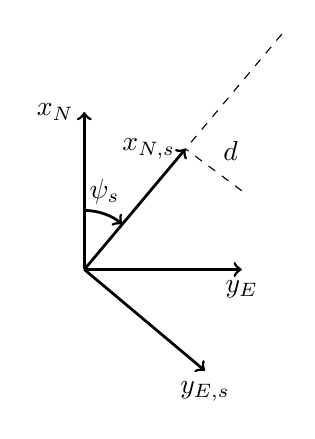
\begin{tikzpicture}
                \Drone{2}{1}{65}
                \coordinate (test) at (50:2);
                \draw[myaxis] (0, 0) -- node[at end, left]{$x_N$} (0, 2);
                \draw[myaxis] (0,0) -- node[at end, below]{$y_E$} (2, 0);

                \draw[myaxis] (0, 0) -- node[at end, left]{$x_{N,s}$} (test);
                \draw[myaxis] (0,0) -- node[at end, below]{$y_{E,s}$} (-40:2);
                \draw[myaxis](0,0.75) arc(90:50:0.75) node[midway, above]{$\psi_s$};
                \draw[dashed](0, 0) -- (50:4);
                \draw[dashed](2,1) -- node[midway, anchor=south west]{$d$} (test);
            \end{tikzpicture}        
    \end{center}
    \caption{Coordinate frame for straight path following}
    \label{fig:coord_straight}
\end{figure}

The relevant equations for the control problem in this frame become
\begin{align}
    \dot{d}\equiv\dot{y}_{E,s} &= V_a\sin(\psi-\psi_s) + W\sin(\psi_w-\psi_s)\\
    \dot{\psi} &= \frac{g}{V_a}\tan\phi
\end{align}
Assuming that $d=0$ and $\dot{d}=0$, we get
\begin{equation}
    V_a\sin(\psi-\psi_s) + W\sin(\psi_w-\psi_s)=0
\end{equation}
This means that the cross-track error is minimized when $\psi$ converges to
\begin{equation}\label{eq:wca}
    \psi_{wca}=-\arcsin\left(\frac{W}{V_a}\sin(\psi_w-\psi_s)\right) + \psi_s
\end{equation}
In the case of no wind, this simplifies to $\psi_{wca}=\psi_s$. In windy conditions however, the wind 
has to be compensated with a constant offset which depends on wind speed, direction and desired 
heading $\psi_s$. $\psi_{wca}$ is called the \textit{wind correction angle} \cite{uav_dynamics_wind}.

\section{ArduPlane autopilot}
The ArduPlane autopilot is an open source autopilot for fixed-wing UAVs \cite{arduplane}. 
It contains high-level controllers for navigation, velocity and altitude control as well as 
low level logic to command the attitude and throttle of the vehicle. In the following section
the underlying theory of the relevant control loops for this thesis will be presented.

\subsection{Trajectory controller}\label{sec:traj_controller}
The ArduPlane autopilot uses the $L_1$ control law described in \cite{arduplane_l1} for trajectory following.
The goal of the control loop is to follow a straight line from a start coordinate $\vec{p}_{s}$ to a goal
coordinate $\vec{p}_{g}$. This is obtained by aiming towards a point $P$ which is located at a
fixed distance $L_1$ from the UAV. 
The logic behind the controller is illustrated in Figure~\ref{fig:ss_defs},
where $\vec{p}$ is the UAV position and $\psi$ is the UAV yaw angle.
\begin{figure}[htb]
    \begin{center}
    \tikzstyle{point} = [
        circle,
        minimum width=3.5pt,
        inner sep=0,
        fill=black
    ]
    \tikzstyle{my_v} = [
        ->,
        line width = 1.2pt
    ]
    \begin{tikzpicture}[scale=0.85]
        %\draw[help lines](0,0) grid (10,10);
        \coordinate (origin) at (1,1);
        \coordinate (drone) at (2,6);
        \coordinate (goal) at (9,9);
        \coordinate (ref) at (7,7);
        
        \node[anchor=300] at (drone) {$\vec{p}$};
        \draw[my_v] (drone) -- node[above, near end, anchor=south east]{$\vec{v}$} ++ ({atan(2)}:2.5);

        \draw[->] (drone) -- node[right, at end]{$a^c$}++ (-45:1);

        \draw[->] ([yshift=0.7cm]drone) arc(90:{atan(2)}:0.7) node[above,midway]{$\psi$};
        \draw[dashed] (drone) --++ (0,1);
        \draw[->] (drone) ++ (0.5,1) arc({atan(2)}:{atan(0.2)}:{sqrt(1.25)}) node[midway,anchor=223]{$\eta$};
        

        \node[anchor=north west] at (origin) {$\vec{p}_s$};

        \node[anchor=north west] at (goal) {$\vec{p}_g$};
        
        \draw (drone) -- node[above,sloped]{$L_1$} (ref);
        \node[point] at (ref) {};
        \node[anchor=north west] at (ref) {$P$};
        
        \draw[] (origin) -- node[above, at end]{} (goal);
        \node[point] at (origin) {};
        \node[point] at (goal) {};
        \node[point] at (drone) {};
    
        \Drone{2}{6}{70};

    \end{tikzpicture}
        
    \caption{$L_1$ controller logic}
    \label{fig:ss_defs}
    \end{center}
\end{figure}

In the ArduPilot implementation, the distance $L_1$ is calculated as
\begin{equation}\label{eq:ardu_l1}
    L_1=\begin{cases}
        \frac{1}{\pi}\zeta\Delta TV & \mbox{if}\quad |\frac{1}{\pi}\zeta\Delta TV|>|\vec{p}_g-\vec{p}| \\
        |\vec{p}_g-\vec{p}| & \mbox{otherwise}
    \end{cases}
\end{equation}
where $V=|\vec{v}|$, $\zeta$ is the damping factor and $\Delta T$ is the update period of the controller \cite{arduplane_l1}.
Wind effects are compensated by using the inertial frame velocity vector 
\begin{equation}
    \vec{v} = V_a\begin{bmatrix}
        \cos\psi \\
        \sin\psi
    \end{bmatrix}
    + W\begin{bmatrix}
        \cos\psi_w\\
        \sin\psi_w
    \end{bmatrix}
\end{equation}
 In each time step, the control law corresponds to following a circular segment with radius
 \begin{equation}
    R=\frac{L_1}{2\sin\eta}
 \end{equation}
 which is tangent to $\vec{v}$ in $(x,y)$.
 $\eta$ is defined as the angle between the UAV velocity vector $\vec{v}$ and the line from the UAV to $P$.
This circular segment is followed by issuing a lateral acceleration command
\begin{equation}\label{eq:lat_acc}
    a^{c}=2\frac{V^2}{L_1}\sin\eta
\end{equation}
The lateral acceleration command is translated to a roll command
\begin{equation}\label{eq:roll_cmd}
    \phi^{c}=\tan^{-1}(a^{c}/g)
\end{equation}
where $g$ is the gravitational constant. The low-level attitude controller is then used to track the desired roll.

In the case of a straight reference trajectory, it is shown in \cite{l1_controller} that \eqref{eq:lat_acc} 
can be linearized to
\begin{equation}
    a^c\approx2\frac{V}{L_1}\left(\dot{d}+\frac{V}{L_1}d\right)
\end{equation} 
which is a PD-controller. Furthermore, if inner-loop dynamics are neglected and 
$\vec{v}$ is assumed parallel to the reference line, $a^c\approx \ddot{d}$ and we get
\begin{equation}
    \ddot{d} + 2\zeta\omega_n\dot{d} + \omega_n^2d=0
\end{equation}
with $\zeta=1/\sqrt{2}$ and $\omega_n=\sqrt{2}V/L_1$. This is a simple second-order system where 
the damping is constant, and the speed depends on the ratio between $V$ and $L_1$. 
\iffalse
\subsection{Altitude and velocity control loop}
ArduPlane uses a combined control loop to handle both desired altitude and velocity, called 
TECS (Total Energy Control System). This controller is based on the total energy of the UAV,
which is defined as
\begin{equation}
    E_T=\frac{1}{2}mV^2 + mgh
\end{equation}
where $h$ is the altitude relative to the takeoff point. The total energy rate is derived
by taking the derivative with respect to time as
\begin{equation}
    \dot{E}_T=mV\dot{V} + mg\dot{h}
\end{equation}
The specific energy rate is then
\begin{equation}
    \dot{E}_S = \frac{\dot{E}_T}{mgV} = \frac{\dot{V}}{g} + \frac{\dot{h}}{V} = \frac{\dot{V}}{g} + \sin\gamma
\end{equation}
If $\gamma$ is small, we get
\begin{equation}
    \dot{E}_S\approx\frac{\dot{V}}{g} + \gamma
\end{equation} 
The longitudinal aircraft dynamics give
\begin{equation}
    T-D=\frac{\dot{V}}{g} + \gamma
\end{equation}
Thus, by increasing the thrust
energy is added to the system. By changing the pitch angle using the elevators, the balance 
between kinetic and potential energy can be modified. 
\fi

\subsection{Mission representation and flight modes}\label{sec:mission}
A \textit{mission} $\mathcal{M}$ is defined as 
\begin{equation}
    \mathcal{M} = \{\vec{p}_1, \hdots, \vec{p}_n\}
\end{equation}
i. e. a sequence of $n$ \textit{waypoints} represented in the inertial frame as 
\begin{equation}
    \vec{p}=(x_N, y_E, -z_H, c_{wp})
\end{equation}
where $c_{wp}$ represents the waypoint command. There are many different waypoint commands available
in ArduPlane, but this work will be focused on 
\begin{equation}
    c_{wp}\in \{Waypoint, Takeoff, Land\}
\end{equation}
\subsubsection{Waypoint mode}
In \textit{waypoint} mode the trajectory following controller is used
to navigate along the line from $\vec{p}_i$ to $\vec{p}_{i+1}$. When $\vec{p}_{i+1}$ is reached, the flight mode
is updated depending on the next $c_{wp}$. The next waypoint is assumed to be reached when
\begin{equation}
    \|\vec{p}_{UAV}-\vec{p}_{wp}\| < R_{wp}
\end{equation}
where $R_{wp}$ is defined by the user, or passed when
\begin{equation}
    \frac{\|\vec{p}_{UAV}\cdot \vec{p}_{wp}\|}{\|\vec{p}_{wp}\|}
     \geq 1
\end{equation}
where $\vec{p}_{UAV}=\vec{p}-\vec{p}_i$ and $\vec{p}_{wp}=\vec{p}_{i+1}-\vec{p}_i$ \cite{ardupilot_auto}.
\subsubsection{Land mode}
In \textit{Land} mode, the plane will attempt to land at a given coordinate. The landing approach 
is divided into two different stages, the \textit{approach} stage and \textit{flare} stage.

During the approach stage, the UAV tries to accomplish the commanded \textit{glide slope}, which is
dependent on the previous waypoint position relative to the landing point. When the altitude decreases
below $h_{flare}$, it enters the flare stage which means the throttle is completely turned off. 
During this stage the UAV will try to hold a target descent rate $\dot{h}_{flare}$ which is
defined by the user \cite{ardupilot_land}.